\subsection{Micro Ampere ASV}
\todo{TAP: Personally, not sure I like starting chapter 3 with a picture. Some into text would be good. Also, I like the when the figures are placed on top of page, not in the middle of the page...}
\begin{figure}[!tbp]
    \centering
    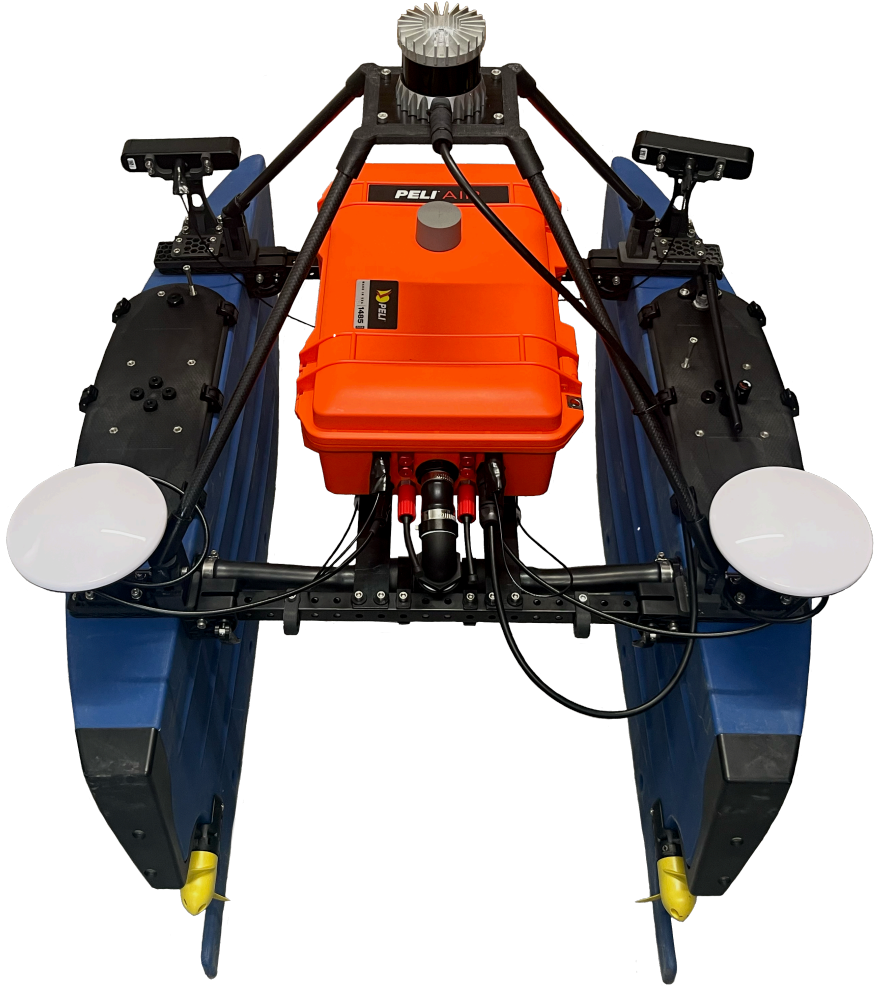
\includegraphics[width=0.6\linewidth]{Pictures/Hardware/microAmpere_ASV/microAmpere_ASV.png}
    \caption{A picture of microAmpere Autonomous Surface Vessel (ASV). Picture taken from Luan Cao Vo Tran master thesis on microAmpere ASV.\textsuperscript{\cite{microAmpere_hardware_master_thesis1}}}
    \label{fig:microAmpere}
    \todo{TAP: add reference to fig, where is the figure taken from? I see you have added a reference as a text, would be better to write someting like: A picure of .... (ASV) [3] , where [3] is the reference number in the bibliography. This applies to all later figures as well.}
\end{figure}
\noindent
This section focuses on the \textit{``microAmpere Autonomous Surface Vessel (ASV)''} platform, which serves as the primary research and development base for this work. The information presented here is summarized from two detailed master theses, Luan Cao Vo Trans thesis on microAmpere hardware and integration \cite{microAmpere_hardware_master_thesis1}, and Henrik Reimers thesis on control and system design \cite{microAmpere_hardware_master_thesis2}. More detailed technical descriptions can be found in the referenced theses.
\\ \\
In this section, only the most relevant aspects of the platform are presented, specifically those that are essential for integrating a side scan sonar payload and for enabling SSS SLAM. The focus is therefore on the hardware architecture, computing layout, and synchronization systems that directly affect sonar data acquisition and processing.
\\ \\
The microAmpere is an advanced Autonomous Surface Vessel (ASV) developed at NTNU as a modular platform for autonomous docking and maritime robotics research. It is part of the Autodocking25 project \todo{TAP: add reference} and represents the next evolution of the Blue Robotics BlueBoat platform. The vessel was redesigned to support high performance perception, navigation, and control tasks under realistic marine conditions. Its main purpose is to provide a flexible and open research platform for experimenting with autonomous operations such as docking, waypoint navigation, and sensor fusion at sea.
\\ \\
Physically, the vessel is based on the BlueBoat twin hull design, offering high stability and sufficient deck space for custom payloads. The hulls are constructed from High Density Polyethylene (HDPE), ensuring durability and resistance to saltwater corrosion. The superstructure houses one watertight enclosures containing the compute units, sensor interfaces, and power management systems. This enclosure is designed for quick maintenance and allows for modular upgrades for new hardware.
\\ \\
The system integrates a distributed computing architecture consisting of a \textit{``Jetson Orin NX''} for GPU intensive perception tasks such as LiDAR and camera processing, and a \textit{``LattePanda 3 Delta''} Single Board Computer (SBC) for real-time navigation, control, and communication handling. Both systems run ROS2 with synchronized clocks via GNSS and PPS hardware timing, achieving sub microsecond precision across devices. This allows accurate sensor timestamping and time alignment between the navigation, control, and perception subsystems.
\\ \\
The sensor suite includes dual GNSS antennas for accurate heading estimation, a high grade IMU for attitude and acceleration measurements, an \textit{``Ouster OS1''} LiDAR for 3D environmental mapping, and \textit{``StereoLabs ZED-X''} stereo cameras for visual perception and teleoperation. A dedicated power sensing board monitors voltage and current to ensure system safety, and an industrial \textit{``Teltonika RUTX50''} router provides 4G/5G and GNSS connectivity, extending operational range far beyond line of sight limits. All components are interconnected through a structured internal wiring system with proper isolation, grounding, and surge protection to handle harsh marine environments.
\\ \\
The MicroAmperes software stack is fully containerized, combining real-time control loops with modular high level autonomy nodes. Each module communicates through standardized ROS2 topics and services, enabling independent algorithm development without system reconfiguration. This architecture also facilitates rapid iteration and field testing of advanced autonomy features such as Model Predictive Control (MPC), Reinforcement Learning (RL), and Simultaneous Localization and Mapping (SLAM).
\\ \\
In addition to autonomy research, the microAmpere platform is used for multi sensor data collection and algorithm benchmarking under controlled sea trials. The synchronized data from LiDAR, stereo vision, IMU, and GNSS enables high quality datasets for perception, sensor fusion, and state estimation studies. The vessels modular interfaces also make it suitable for integration with experimental payloads such as side scan sonar, underwater acoustic systems, or alternative control computers for specific research tasks.
\\ \\
From a systems engineering perspective, microAmpere demonstrates the effectiveness of distributed embedded computing in marine robotics. By separating perception and control workloads, developers can independently optimize performance for GPU heavy machine learning pipelines and deterministic control processes. The modular ROS2 setup also supports simulation-in-the-loop and hardware-in-the-loop testing, ensuring smooth transition from virtual models to field deployment.
\\ \\
According to Luan Cao Vo Tran master thesis on microAmpere ASV \cite{microAmpere_hardware_master_thesis1} and Henrik Reimers master thesis on microAmpere ASV \cite{microAmpere_hardware_master_thesis2}, the platform has already undergone multiple field campaigns in Trondheim Fjord. These tests validated microAmpere ASVs hardware robustness, networking reliability, and autonomy stack. Its success has positioned it as a reference platform for NTNUs future autonomous surface vessel research, bridging efforts between the Department of Cybernetics and the AUR Lab. 
\\ \\
Overall, the microAmpere ASV serves as a compact but powerful research platform, bridging the gap between simulation and real world autonomous marine systems. Its modular design, distributed computation, and precise timing infrastructure make it ideal for experimentation with advanced autonomy, perception, and control algorithms in challenging maritime environments.
